\documentclass[12pt,onecolumn,a4paper]{article}
\usepackage{epsfig,graphicx,amsthm,amsmath}
\usepackage{color,xcolor}
\usepackage{pgfplots}
\pgfplotsset{compat=newest}
\usepackage{tikz}
\usepackage{caption}
\usepackage{subcaption}
\usepackage{multirow}
\usepackage{xepersian}
\settextfont{XB Zar}
\setlatintextfont{Times New Roman}

\newtheorem{theorem}{قضیه}[section]
\newtheorem{corollary}{نتیجه‌}[theorem]

\pgfplotstableread[col sep = comma]{gibbs.csv}\gibbs
\pgfplotstableread{
-1 0
-1 -1
0 -1
0 1
1 1
1 0
}\gibbsref
\pgfplotstableread[col sep = comma]{adv_phenom_oned.txt}\signoned
\pgfplotstableread[col sep = comma]{adv_phenom_mono.txt}\signmono
\pgfplotstableread[col sep = comma]{adv_phenom_cheby.txt}\signcheby
\pgfplotstableread[col sep = comma]{adv_phenom_legen.txt}\signlegen
\pgfplotstableread[col sep = comma]{adv_phenom_samples.txt}\signmemory

\begin{document}
\title{توجیه وجود مثال‌های خصمانه \\ و انتقال‌پذیری آن‌ها} 
\author{رامین براتی}
\date{\today}
\maketitle

\begin{abstract}
یادگیری عمیق در مرکز پیشرفت‌های اخیر در یادگیری ماشین و هوش مصنوعی قرار دارد. با این که این مدل‌ها توانایی فراانسانی در انجام بعضی کاربردها از خود نشان می‌دهند، مطالعات نشان داده است که این مدل‌ها به تغییرات کوچک و غیر قابل تشخیص در ورودی حساس هستند. این اختلالات را اختلالات خصمانه نام‌گذاری کرده‌اند. پدیده‌ی اختلالات خصمانه تهدید قابل توجهی برای استفاده از مدل‌های یادگیری ماشین در کاربردهای نیازمند ایمنی است و به همین دلیل، تحقیقات بسیاری در این مسیر انجام شده است. در این مقاله، دیدگاه جدیدی در مورد دلیل وجود این پدیده ارائه می‌دهیم. با تکیه بر این دیدگاه، روشی برای ایمن‌سازی شبکه‌های عصبی به حملات گرادیان-پایه ارائه می‌دهیم. نتایج اولیه حاکی از موثر بودن روش پیشنهادی در کاهش قابل توجه حساسیت شبکه‌های عصبی به مثال‌های خصمانه است. در عین حال، پیاده‌سازی روش پیشنهادی وابستگی‌ای به شبکه‌های عصبی ندارد و به راحتی قابل انتقال به دیگر مدل‌های یادگیری ماشین نیز هست.
\end{abstract}

\section{مقدمه} 
با پیشرفت‌هایی که اخیرا در الگوریتم‌ها و قدرت محاسباتی به وجود آمده، یادگیری ماشین به یکی از پرکاربردترین ابزارها در صنایع مختلف تبدیل شده است. بدون شک، ظهور و معرفی آموزش عمیق به همراه وجود مجموعه‌های بزرگ آموزشی را می‌توان مسئول بخش قابل توجهی از این پیشرفت‌ها دانست. موفقیت‌ کاربرد آموزش عمیق در مسائل طبقه‌بندی تصاویر، شناسایی اشیا، پردازش زبان طبیعی و دیگر کاربردهای متنوع جایگاه شبکه‌های عصبی چندلایه در صنایع مختلف را نیز تثبیت کرده است.

با توجه به این پیشرفت‌ها، طبیعی است که بخواهیم از این مدل‌ها در کاربردهایی مانند ماشین‌های خودران و دیگر کاربردهایی که امنیت در آنها اهمیت دارد استفاده کنیم. با این حال، در
\cite{szegedy2013intriguing} 
نشان داده شد که مدلهای عمیق به پدیده‌ی مثال‌های خصمانه حساس هستند. مثال‌های خصمانه نقاطی در همسایگی مثال‌های طبیعی هستند که طبقه‌بند در آن نقاط خروجی اشتباه می‌دهد. در بعضی از موارد، تفاوت میان مثال خصمانه با مثال طبیعی برای انسان قابل تشخیص نیست.

انتظار می‌رود که در آینده‌ی نزدیک، مدل‌های عمیق بسیاری در دنیای فیزیکی تعیبیه شوند. در عین حال، مطالعات و تحقیقات اخیر نشان می‌دهند که مثال‌های خصمانه را در دنیای واقعی نیز می‌توان به کار برد. برای مثال، می‌توان ورودی را به گونه‌ای تغییر داد که دستگاه‌هایی که برای گرفتن دستورات از مدل‌های شناسایی گفتار استفاده می‌کنند دستورات اشتباهی را اجرا کنند و یا باعث شد که ماشین‌های خودران در شناسایی عابران پیاده دچار اشتباه شوند. این مسئله، نگرانی‌های بسیاری را در مورد ایمنی استفاده از مدل‌های یادگیری ماشین و شبکه‌های عمیق به وجود آورده است.

در کاربردها، شبکه‌های عصبی عمیق را به صورت مدلهای جعبه سیاه در نظر می‌گیرند. به این معنی که می‌دانیم که این مدل‌ها عملکرد خوبی دارند، ولی به طرز کار درونی آن‌ها وقوف نداریم. دلیل وجود مثال‌های خصمانه یکی از پایه‌ای‌ترین مسائل  مطرح در این زمینه است. با این حال، عدم وجود درک کامل از ساز و کار این مدل‌ها و سختی‌های مرتبط با کار در فضاهای بعد بالا، توضیح و تشریح این دلایل را مشکل کرده است. دلیل وجود این پدیده هنوز یک مسئله‌ی باز است و ما خواننده را به \cite{Yuan_2019} برای مطالعه‌ی بیشتر در مورد این پدیده ارجاع می‌دهیم.

در این مقاله، ما دیدگاه جدیدی در مورد دلیل به وجود آمدن پدیده‌ی مثال‌های خصمانه در شبکه‌های عصبی را ارائه داده و مسیر جدیدی را برای مقابله با تاثیرات این پدیده ارائه می‌کنیم. این مقاله در پنج بخش تنظیم شده است. پس از مقدمه، در بخش دوم، مروری بر تعدادی از دیدگاه‌های ارائه شده‌ی مرتبط با دیدگاه پیشنهادی خواهیم داشت. سپس، در بخش سوم، دیدگاه پیشنهادی را تشریح می‌دهیم. در بخش چهارم، شواهدی  در تایید دیدگاه پیشنهادی ارائه داده و بخش پنجم را نیز به جمع‌بندی و تعیین قدم‌های بعدی در این مسیر اختصاص داده‌ایم.

\section{کارهای مرتبط}
تاکنون، برای وجود مثال‌های خصمانه سه دلیل ارائه شده است. اولین دیدگاه توسط سجدی و همکاران\cite{szegedy2013intriguing}
مطرح شد. این دیدگاه، که با نام دیدگاه پاکت‌های نادر شناخته می‌شود، به شرح زیر است. در این دیدگاه، دلیل وجودی مثال‌های خصمانه وجود پاکت‌هایی در فضای ورودی شبکه هستند که احتمال مشاهده‌ی آنها بسیار کم است و شبکه در آن نواحی خروجی مناسبی نمی‌دهد. در این دیدگاه رابطه‌ی مثال‌های خصمانه با فضای ورودی شبکه را مشابه رابطه‌ی میان اعداد گویا و اعداد حقیقی می‌دانند. به این معنی که، احتمال گویا بودن یک نمونه‌ی تصادفی از یک بازه از اعداد حقیقی صفر است، با این وجود در همسایگی هر عدد حقیقی عددی گویا یافت می‌شود. با این حال،
همان گونه که در
\cite{tanay2016boundary}
نیز به آن اشاره شده است، دلیل محکمی برای نشان دادن چنین رفتاری توسط شبکه ارائه نشده است و صرفا به مرتبط کردن آن به بسیار غیرخطی بودن نمایش یادگیری شده توسط شبکه اکتفا شده است. در 
\cite{Tabacof_2016}
 نیز شواهدی ارائه شده است که طبق این شواهد، مثال‌های خصمانه الزاما به صورت ایزوله در فضا پخش نمی‌شوند و نواحی چگال و فشرده‌ای از این مثال‌ها نیز وجود دارد. این دیدگاه چگونگی انتقال این مثال‌ها به شبکه‌های دیگر را نیز مشخص نمی‌کند.

دیدگاه دوم توسط گودفلو و همکاران\cite{goodfellow2014explaining}
مطرح شده است. این دیدگاه، که با نام دیدگاه خطی بودن شناخته می‌شود، هم اکنون مقبول‌ترین دیدگاهی است که در این زمینه ارائه شده است. طبق این دیدگاه، پدیده‌ی مثال‌های خصمانه در طبقه‌بندهای خطی در ابعاد بالا ظهور می‌کند و دلیل مشاهده‌ی این پدیده در شبکه‌های عصبی نیز مرتبط با علاقه‌ی ما در استفاده از الگوهای خطی در مدلسازی و آموزش این شبکه‌ها می‌باشد. گودفلو و همکاران با استفاده از این دیدگاه حمله‌ی
\lr{FGSM}
را طراحی کردند که از این خطی بودن شبکه‌های عصبی برای تولید مثال‌های خصمانه استفاده می‌کند. ضرب داخلی بین یک بردار وزن $w$ و یک مثال خصمانه‌ی $\tilde{x}=x+\eta$ را در نظر بگیرید.
\begin{equation*}
w^T\tilde{x}=w^Tx+w^T\eta
\end{equation*}
طبق معادله، اگر $\eta$ را برابر با $\mathrm{sign}(w)$ در نظر بگیریم، بیشترین تغییر را، تحت قید نورم ماکزیموم، در خروجی اعمال کرده‌ایم. خطی بودن به این معناست که شبکه رفتاری مشابه از خود نشان داده و در صورتی که $\eta$ را برابر با علامت گرادیان تابع هزینه در نقطه‌ی $x$ قرار دهیم، شبکه در طبقه‌بندی دچار خطا خواهد شد.

طبق این دیدگاه، دلیل انتقال مثال‌های خصمانه به دیگر شبکه‌ها، همگرایی این مدل‌ها به طبقه‌بند خطی بهینه است. دیدگاه خطی بودن دو پیش بینی مستقیم دارد، اول این که تمامی طبقه‌بندهای خطی از پدیده‌ی مثال‌های خصمانه رنج می‌برند و دوم این که اثر خطی بودن با افزایش ابعاد مسئله تشدید می‌شود. با این وجود، در
\cite{tanay2016boundary}
هر دوی این پیش‌بینی‌ها زیر سوال می‌روند. ابتدا مسئله‌ای  مصنوع را در نظر می‌گیرند که برای آن طبقه‌بندی خطی وجود دارد که از مثال‌های خصمانه آزاد است و در ادامه نشان می‌دهند که در یک مسئله‌ی واقعی نیز با افزایش ابعاد قدرت مثال‌های خصمانه تشدید نمی‌شود.

دیدگاه سوم توسط تانای و همکاران
\cite{tanay2016boundary}
 و با نام دیدگاه کجی مرز ارائه شده است. این دیدگاه برای طبقه‌بندهای خطی پیشنهاد شده و ظهور آن در شبکه‌های عصبی را منتج از شکلی غیرخطی از این پدیده می‌دانند. یک مسئله‌ی طبقه‌بندی دو کلاسی را در نظر بگیرید که برای آن یک طبقه‌بند خطی را آموزش داده‌ایم. این طبقه‌بند خطی یک مرز تصمیم
 $c$
 برای جدا کردن دو کلاس می‌یابد. حال طبقه‌بند بهینه‌ای را برای همان مسئله در نظر بگیرید که توسط مرکزهای دو کلاس تعریف شده باشد. این طبقه‌بند نیز یک مرز تصمیم
 $c^*$
 برای جدا کردن دو کلاس تعریف می‌کند. طبق دیدگاه کجی مرز در صورتی که مرز
 $c$
 با
 $c^*$
 زاویه داشته باشد، برای طبقه‌بند مثال‌های خصمانه وجود خواهد داشت. تانای و همکاران در ادامه نشان می‌دهند که می‌توان زاویه‌ی بین دو مرز را با منظم کردن\LTRfootnote{regularize}
طبقه‌بند کاهش داد. در پایان، تانای و همکاران با توجه به نوع و شکل اختلالات خصمانه‌ای که در شبکه‌های عصبی مشاهده می‌کنند، دلیل وجود مثال‌های خصمانه برای این شبکه‌ها را منظم نبودن این شبکه‌ها اعلام می‌کنند. با این که تانای و همکاران دلایل خوبی در تایید دیدگاه کجی مرز ارائه می‌دهند، چگونگی تعمیم آن به شبکه‌های عصبی و دیگر مدل‌های غیرخطی را مشخص نمی‌کنند. همچنین، در این دیدگاه دلیلی برای انتقال‌پذیری مثال‌های خصمانه ارائه نشده است.

همان گونه که مشاهده می‌شود، هیچ‌کدام از دیدگاه‌های مطرح شده توانایی توجیه و تشریح تمامی مشاهدات مرتبط با مثال‌های خصمانه را ندارند. با این حال، هرکدام بخش محدودی از مشاهدات را توجیه می‌کنند. در اینجا، دیدگاه جدیدی را مطرح می‌کنیم که توانایی توجیه وجود مثال‌های خصمانه و انتقال‌پذیری آن‌ها را دارد و  در عین حال، با مشاهداتی که توسط دیدگاه‌های قبلی مطرح شده نیز سازگازی دارد. در ادامه، این دیدگاه جدید را شرح می‌دهیم.

\section{پدیده‌ی رونگه و مثال‌های خصمانه}
در این بخش، دیدگاه جدیدی را در مورد دلیل وجود مثال‌های خصمانه و انتقال‌پذیری آن‌ها ارائه می‌دهیم. در این دیدگاه مثال‌های خصمانه نتیجه‌ی پدیده‌ای مشابه پدیده‌ی رونگه هستند و انتقال‌پذیری آن‌ها متاثر از روابط موجود بین ابعاد مثال‌های طبیعی در فضای ورودی و وجود تکینگی در تابع هدف است. ابتدا پدیده‌ی رونگه را شرح می‌دهیم.

در آنالیز عددی، پدیده‌ی رونگه مشکلی است که هنگام درون‌یابی با استفاده از چندجمله‌ای‌های درجه بالا با استفاده از نقاط هم فاصله به وجود می‌آید. طبق قضیه‌ی تقریب وایرشتراس\LTRfootnote{Weierstrass approximation theorem}،
هر تابع پیوسته‌ی 
$f(x)$
که بر روی یک بازه‌ی
$[a,b]$
تعریف شود را می‌توان با استفاده از یک چندجمله‌ای درون‌یاب
$P_n(x)$
تقریب زد. به عبارت دقیق‌تر
\begin{equation*}
    \lim_{n\rightarrow \infty}\left(\max _{{a\leq x\leq b}}\left|f(x)-P_{n}(x)\right|\right)=0.
\end{equation*}
طبق این قضیه، طبیعی است که انتظار داشته باشیم که با افزایش 
$n$
به تقریب دقیق‌تری از تابع مورد نظر دست یابیم. با این وجود، ممکن است که دنباله‌ی چندجمله‌ای‌هایی که انتخاب شده‌اند خاصیت همگرایی یکپارچه را نداشته باشند. توجه کنید که قضیه‌ی تقریب وایرشتراس فقط وجود این چندجمله‌ای را تضمین می‌کند، و مسیری برای یافتن این چندجمله‌ای مشخص نمی‌کند. در واقع، چندجمله‌ای‌هایی که ساخته می‌شوند ممکن است با افزایش درجه‌ی چندجمله‌ای واگرا شوند. پدیده‌ی رونگه به صورت الگوهای نوسانی بروز کرده که در نزدیکی نقاط درون‌یابی انتهایی بازه افزایش می‌یابد و نشان از نامناسب بودن نقاط درون‌یابی هم فاصله برای انجام درون‌یابی دارد. شناسایی این پدیده را به  کارل رونگه\LTRfootnote{Carl David Tolme Runge}،
ریاضیدان آلمانی، منتصب می‌کنند.

تابع رونگه با تعریف 
$f(x)=\frac{1}{1+25x^2}$ 
را در نظر بگیرید. چندجمله‌ای درون‌یاب این تابع را با استفاده از نقاط 
$x_i$ 
، به طوری که
$x_{i}=\frac{2i}{n}-1$ 
و 
$i\in \left\{0,1,\dots ,n\right\}$،
تعریف می‌کنیم.
همان گونه که مشاهده می‌شود، نقاط 
$x_i$ 
در بازه‌ی 
$[-1,1]$ 
و با فاصله‌ی یکسان توزیع شده‌اند. رونگه متوجه شد که چندجمله‌ای درون‌یابی که به روش ذکر شده ساخته شود، در نزدیکی مرز‌های دامنه‌ی تابع نوسان می‌کند. حتی می‌توان نشان داد که خطای درون‌یابی با افزایش 
$n$ 
 به صورت بیکران افرایش می‌یابد.

پدیده‌ی رونگه هنگام درون‌یابی با استفاده از پایه‌های تک‌جمله‌ای\LTRfootnote{Monomial basis} 
بروز پیدا می‌کند. با این حال تغییر این توابع پایه برای حل مسئله کافی نیست. اگر از توابع پایه‌ی مثلثاتی، مثلا توابع پایه‌ی فوریه، برای تشکیل چندجمله‌ای درون‌یاب استفاده کنیم، با مشکل مشابهی مواجه می‌شویم. این مشکل  با نام پدیده‌ی گیبس\LTRfootnote{Gibbs phenomenon}
شناخته می‌شود. پدیده‌ی گیبس باعث به وجود آمدن نوساناتی در نزدیکی ناپیوستگی‌های تابع شده و این امر موجب فراجهش
در این نقاط می‌شود. در نتیجه، در صورتی که تابعی که قصد تقریب زدن آن را داریم متناوب نباشد، این تقریب از تابع نیز در نزدیکی مرزها دچار نوسان خواهد شد. در شکل 
\ref{fig:runge_gibbs} 
این دو پدیده با مثال‌هایی نشان داده‌ شده‌اند.

 \begin{figure}
    \centering
    \begin{subfigure}[b]{0.45\textwidth}
        \centering
        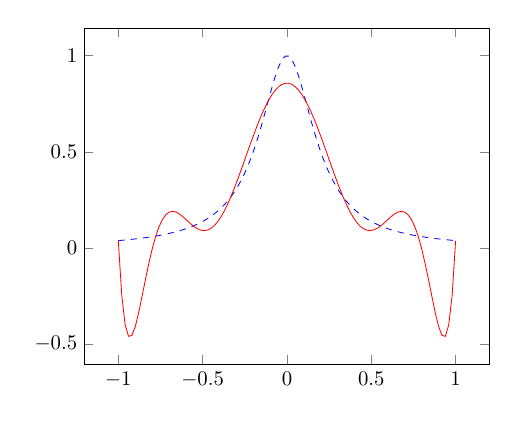
\begin{tikzpicture}[scale=0.75]
            \begin{axis}[xmin=-1,xmax=1,xmin=-1.2,xmax=1.2,samples=100]
                \addplot[domain=-1:1,blue,dashed]{1/(1+25*x*x)};
                \addplot[domain=-1:1,red,solid]{16.545674722429712 * x*x*x*x*x*x*x*x*x*x + 8.851286807773627e-13 * x*x*x*x*x*x*x*x*x + -12.079377458718012 * x*x*x*x*x*x*x*x + -1.6319051537287015e-12 * x*x*x*x*x*x*x + -22.778903788331114 * x*x*x*x*x*x + 8.747268893200492e-13 * x*x*x*x*x + 25.348331583973515 * x*x*x*x + -1.4087385060936399e-13 * x*x*x + -7.854564043148674 * x*x + 6.6005027351349585e-15 * x + 0.8573005222561162};
            \end{axis}
         \end{tikzpicture}
        \caption{پدیده‌ی رونگه}
        \label{fig:runge}
    \end{subfigure}
    \hfill
    \begin{subfigure}[b]{0.45\textwidth}
        \centering
        \begin{tikzpicture}[scale=0.75]
            \begin{axis}[xmin=-1,xmax=1,xmin=-1.2,xmax=1.2,samples=100]
                \addplot[mark=none,blue,dashed] table{\gibbsref};
                \addplot[mark=none,red,solid] table{\gibbs};
            \end{axis}
         \end{tikzpicture}
        \caption{پدیده‌ی گیبس}
        \label{fig:gibbs}
    \end{subfigure}
       \caption{دو پدیده‌ی رونگه و گیبس. در هر دو نمودار خم آبی تابع هدف و خم قرمز تقریب متناظر با آن تابع می‌باشد. (آ) تابع رونگه و تقریب آن توسط یک چندجمله‌ای درجه 10. (ب) تابع پله‌ای و تقریب آن با استفاده از 30 جمله‌ی اول سری فوریه‌ی متناظر آن.}
       \label{fig:runge_gibbs}
\end{figure}

تا کنون برای کاهش پدیده‌ی رونگه چند روش عمده پیشنهاد شده است. شناخته‌ترین روش استفاده از نقاط درون‌یابی غیر هم‌فاصله، مانند گره‌های چبیشف، است. دو روش عمده‌ی دیگر، روش‌های کمترین مربعات و منظم‌سازی هستند. در روش کمترین مربعات، یک چندجمله‌ای درجه پایین‌تر را به مجموعه‌ی نقاط درون‌یابی برازش می‌دهند. در مقابل، در روش منظم‌سازی یک چندجمله‌ای درجه بالاتر را از نقاط عبور داده و از بقیه‌ی درجه‌های آزادی برای ارضای هدف منظم‌سازی استفاده می‌کنند.

طبق تئوری تقریب جهانی، هر تابع پیوسته‌ی $f(x)$ که بر روی بازه‌ی $[a,b]$ تعریف شود را می‌توان، با رعایت نکاتی در مورد تابع فعال‌سازی، توسط یک شبکه‌ی عصبی سه لایه تقریب زد. با مقایسه‌ی این قضیه و قضیه‌ی تقریب وایرشتراس می‌توان مشاهده کرد که این قضیه نیز فقط وجود این شبکه را تضمین می‌کند و روشی برای پیدا کردن این شبکه مشخص نمی‌کند. در واقع، تضمینی وجود ندارد که الگوریتم آموزش توانایی یافتن وزن‌های مناسب را داشته باشد. در اینجا، ما نشان می‌دهیم که مجموعه‌های آموزشی مصنوعی می‌توان ساخت که فرآیند آموزش با الگوریتم بازگشت به عقب، در یافتن وزن‌های مناسب برای شبکه شکست بخورد.

پدیده‌ی یافت شده ارتباطی غیر بدیهی با ابعاد ورودی و روابط و وابستگی‌های بین آن‌ها و چگالی مثال‌های آموزشی در فضای ورودی دارد. برای نشان دادن این پدیده از تابع $\mathrm{sign}(x)$ استفاده می‌کنیم. در شکل (شکل) این تابع، به همراه یک شبکه‌ی چند لایه که به این تابع برازش داده شده، نشان داده شده است. همان گونه که مشاهده می‌شود، شبکه‌ی یافت شده تابعی صاف است و جانشین قابل قبولی برای یک طبقه‌بند خواهد بود. حال، با استفاده از توابع پایه‌ی تک‌جمله‌ای، چبیشف و لژاندر ابعاد ورودی را گسترش می‌دهیم. از آنجایی که با صفر قرار دادن ضرایب ابعاد اضافه شده در نورون‌ها، در عمل، شبکه‌ی اصلی را باز می‌یابیم، می‌توانیم با اطمینان بگوییم که شبکه‌ی مناسبی برای ورودی گسترش یافته نیز وجود دارد. با این حال، بر خلاف انتظار، الگوریتم انتشار به عقب ممکن است در یادگیری تابع مورد نظر با استفاده از این مجموعه‌های آموزش گسترش یافته شکست بخورد.

در شکل (شکل) نتیجه‌ی آموزش با الگوریتم انتشار به عقب در هر سه حالت گسترش ابعاد نشان داده شده است. همان گونه که مشاهده می‌شود، هنگامی که ابعاد را با استفاده از توابع پایه‌ی چبیشف افزایش می‌دهیم، خروجی شبکه در مناطقی که مثالی در آنجا ندیده است دچار نوسانات شدید می‌شود. این نوسانات در صورت استفاده از توابع لژاندر نیز وجود دارند ولی اندازه‌ی آن‌ها نسبت به چبیشف بسیار کمتر است. در مقابل، استفاده از توابع پایه‌ی تک‌جمله‌ای نوسانی به خروجی شبکه وارد نمی‌کند. این مشاهدات با انتظار اولیه‌ی ما تفاوت دارند زیرا توابع چبیشف و لژاندر، برعکس تک‌جمله‌ای‌ها، پایه‌های عمود و نورمال شده‌ای برای چندجمله‌ای‌های روی بازه‌ی $[-1,1]$ هستند.

نتایج به دست آمده مستقل از اندازه‌ی شبکه هستند و به نظر می‌رسد که تنها عامل تعیین کننده در نتیجه‌ی آموزش تعداد و وابستگی‌های میان ابعاد ورودی است. این نتایج نشان می‌دهد که تکیه بر تئوری تقریب جهانی و منظم‌سازی برای موفقیت الگوریتم انتشار به عقب کافی نیست و هنگامی که تعداد ابعاد از یک بزرگتر باشد، شرایطی علاوه بر شرایط خواسته شده در تئوری تقریب جهانی لازم است.

\begin{figure}
	\centering
	\begin{subfigure}[b]{0.45\textwidth}
		\centering
		\begin{tikzpicture}[scale=0.75]
		\begin{axis}[ymin=-2, ymax=2]
		\addplot[only marks,blue] table{\signmemory};
		\addplot[mark=none,blue,solid] table{\signoned};
		\end{axis}
		\end{tikzpicture}
		\caption{یک بعدی}
		\label{fig:pointwise}
	\end{subfigure}
	\hfill
	\begin{subfigure}[b]{0.45\textwidth}
		\centering
		\begin{tikzpicture}[scale=0.75]
		\begin{axis}
		\addplot[mark=none,red,solid] table{\signcheby};
		\addplot[mark=none,blue,solid] table{\signlegen};
		\addplot[mark=none,black,solid] table{\signmono};
		\end{axis}
		\end{tikzpicture}
		\caption{چند بعدی}
		\label{fig:pointwise_cls}
	\end{subfigure}
	\caption{دو نمونه از شبکه‌های درون‌یاب  برای نقاط درون‌یابی هم فاصله و طبقه‌بند منتج از  این شبکه‌ها (آ) مقایسه‌ی انتخاب تصادفی و مرتب شده‌ی نورون‌های پایه.  (ب) طبقه‌بند حاصل از شبکه‌ی درون‌یاب تصادفی.}
	\label{fig:phenom_nn}
\end{figure}

رفتار شبکه در این نواحی بسیار مشابه رفتار شبکه‌هایی است که از پدیده‌ی مثال‌های خصمانه رنج می‌برند. همان طور که مشاهده می‌شود، این نواحی با مکان واقعی مرز تصمیم فاصله‌ی زیادی دارند. با این وجود، در صورتی که از بعضی مثال‌های طبیعی شروع و با استفاده از شهود جهت گرادیان تابع هزینه‌ی طبقه‌بندی، یعنی $N_n(x)\mathrm{sign}(x)$، قصد یافتن مکان مرز تصمیم را داشته باشیم، به اشتباه مکان مرز تصمیم را در نزدیکی این مثال‌ها تخمین می‌زنیم.

حال فرض کنید که قصد یادگیری تابع $f$ را با شبکه‌ی $N_n(x)$ داشته باشیم و نقاط هم فاصله را این بار به عنوان مجموعه‌ای از مثال‌های طبیعی یادگیری در نظر بگیرید. تمامی شبکه‌های درون‌یاب این نقاط تابع هدف آموزش را کمینه خواهند کرد. اکثر این شبکه‌ها از پدیده‌ی مثال‌های خصمانه رنج می‌برند و وجود این شبکه‌ها در فرآیند آموزش اخلال ایجاد می‌کند. در نتیجه، به روشی برای یافتن شبکه‌ی مورد نظر خود نیاز داریم. در اینجا نیز روش عمده مقابله با این پدیده استفاده از کمترین مربعات و منظم‌سازی است. اگر با منظم‌سازی قصد کاهش پدیده‌ی مثال‌های خصمانه را داشته باشیم باید تعداد نورون‌های شبکه را افزایش دهیم. با این وجود، در حال حاضر روش مشخصی برای عبور دادن شبکه از مجموعه‌ی یادگیری و بهینه‌سازی همزمان تابع منظم‌سازی پیشنهاد نشده است. در مقابل، در صورتی که بخواهیم پدیده‌ی مثال‌های خصمانه را با استفاده از کمترین مربعات کاهش دهیم، لازم است مثال‌های آموزشی خیالی تولید و به مجموعه‌ی آموزشی اضافه کنیم و سپس با استفاده از مجموعه‌ی آموزشی افزوده $N_n(x)$ را آموزش دهیم. از این منظر، آموزش خصمانه را می‌توان روشی برای افزودن مجموعه‌ی آموزشی با نمونه‌های خیالی تعبیر کرد.

دیدگاه پیشنهاد شده در توصیف پدیده‌ی مثال‌های خصمانه با دیدگاه‌های مطرح شده‌ی قبلی اشتراکاتی دارد. در دیدگاه جدید، پدیده‌ی مثال‌های خصمانه از بسیار غیرخطی بودن شبکه‌های عصبی نتیجه می‌شود و از این لحاظ با دیدگاه پاکت‌های نادر سازگار است. در مقابل، با اقتباس از مثال مجموعه‌های اعداد، در دیدگاه جدید مثال‌های طبیعی نقشی مانند اعداد صحیح را بازی می‌کنند و خود این مثال‌ها، و متعاقبا مثال‌های خصمانه، در دامنه‌ی ورودی چگال نیستند. به این معنی که، طبقه‌بندی در نقاط منظمی به درستی اتفاق می‌افتد ولی اگر در خلاف جهت گرادیان از بعضی از این مثال‌ها دور شویم، پاسخ طبقه‌بند بدون گذشتن از مرز تصمیم واقعی تغییر می‌کند.

در دیدگاه جدید، پدیده‌ی مثال‌های خصمانه با نوع همگرایی شبکه‌های عصبی چند لایه ارتباط تنگاتنگی دارد. در حقیقت، شواهد نشان می‌دهند که شبکه‌های عصبی تصادفی هنگام درون‌یابی به صورت یکنواخت همگرا نمی‌شوند. در نتیجه، شبکه‌های حاصل الزاما خواص توابع فعال‌سازی استفاده شده، از جمله پیوستگی و مشتق‌پذیری، را از خود نشان نخواهند داد. در واقع، دیدگاه خطی بودن اثر جانبی محدود کردن بسط تیلور تابع به جمله‌ی خطی است. از این لحاظ، دیدگاه جدید نیز وجود حمله‌ی
\lr{FGSM}
را پیش‌بینی می‌کند. بسط تیلور تابع $f(x)$ حول مثال خصمانه‌ی $\tilde{x}=x+\eta$ به صورت زیر است.
\begin{equation*}
f(\tilde{x})=f(x)+\eta^T\nabla f(x) + O(\|\eta\|^2)
\end{equation*}
از آنجایی که شبکه‌ی عصبی تقریب ما از تابع $f$ است، ممکن است بتوانیم شبکه را به عنوان جانشین $f$ در نظر بگیریم. منتهی، از آنجایی که همگرایی به صورت نقطه‌ای اتفاق افتاده است، دلیلی برای برابر بودن گرادیان شبکه‌ی عصبی با گرادیان $f$ وجود ندارد و نباید انتظار داشت که محاسبات بالا، حتی در صورت استفاده از مشتقات مراتب بالاتر، با مقدار واقعی $f(\tilde{x})$ برابر شود. همچنین، در دیدگاه جدید، دلیل انتقال‌پذیری مثال‌های خصمانه همگرایی فرآیند آموزش به میانگینی از شبکه‌های درون‌یاب مجموعه‌ی مثال‌های طبیعی آموزشی در نظر گرفته شده است که با دلیل ارائه شده در دیدگاه خطی بودن تفاوت کوچک ولی مهمی دارد. به عبارت دقیق‌تر، توزیع مثال‌های طبیعی کم و بیش منظم است و طبق نتایج به دست آمده در 
\cite{doi:10.1137/090774707}، 
نقاط هم فاصله، فارق از روش تقریب، برای تقریب توابع مناسب نیستند.

همان گونه که اشاره شد، دیدگاه کجی مرز برای طبقه‌بندهای خطی ارائه شده است. در مقابل، دیدگاه پیشنهادی فقط برای طبقه‌بندهای غیرخطی معتبر است. آز آنجایی که هر طبقه‌بند خطی را می‌توان با استفاده از یک طبقه‌بند غیرخطی نیز نشان داد، پس طبقه‌بندهای غیرخطی نسبت به اثرات هر دو دیدگاه حساس هستند. خوشبختانه، به نظر می‌رسد که روش‌های مقابله با هر دوی این منابع خطا مشابه بوده و احتمالا بهبود در یکی از این دیدگاه‌ها باعث بهبود در دیگری نیز خواهد شد. با این وجود، اجماع این دو دیدگاه نشان از این موضوع دارد که دلیل یکتایی برای وجود مثال‌های خصمانه وجود ندارد. مثال‌های خصمانه ممکن است به طرق متفاوتی به وجود آمده و برطرف کردن یکی از این دلایل الزاما باعث از میان رفتن پدیده‌ی مثال‌های خصمانه نخواهد شد.

\section{شواهد و آزمایش‌ها}
در این بخش، شواهدی در تایید رابطه‌ی پدیده‌ی مثال‌های خصمانه و دیدگاه پیشنهادی را ارائه می‌دهیم. همان گونه که در بخش قبل به آن اشاره شد، طبق دیدگاه پیشنهادی، دو روش عمده‌ی مقابله با پدیده‌ی مثال‌های خصمانه منظم‌سازی و روش کمترین مربعات است. با این  حال، وجود این رابطه را بدون استفاده از روش‌های اشاره شده نیز می‌توان نشان داد. با تکیه بر دیدگاه پیشنهادی، هنگام طبقه‌بندی تصاویر با استفاده از شبکه‌های عصبی، می‌توان قید بسیار قویی به شبکه اضافه کرد که شبکه را نسبت به تمامی حملات مبنی بر شهود گرادیان  شبکه، از جمله حمله‌ی \lr{FGSM}، ایمن کند.

می‌دانیم که، در کاربرد طبقه‌بندی تصاویر، دامنه‌ی ورودی شبکه ابرمکعب $[-1,1]^D$ است و $D$ بعد ورودی را نشان می‌دهد. در این کاربرد، می‌توان فرض کرد که برچسب هر نقطه با برچسب نزدیکترین نقطه روی سطح ابرمکعب برابر است. نزدیک‌ترین نقطه روی سطح ابرمکعب به مثال طبیعی را می‌توان با نورمال کردن مقادیر پیکسل‌ها، به گونه‌ای که بزرگترین مقدار مطلق پیکسل‌ها برابر با یک شود به دست آورد. در داده‌های آموزشی ساده‌تر، مانند 
\lr{MNIST}، 
می‌توان فرض کرد که برچسب هر نقطه‌ی روی سطح ابرمکعب با برچسب نزدیکترین گوشه برابر است. در نتیجه، تعداد مثال‌های طبیعی حداکثر به تعداد گوشه‌های این ابرمکعب، یعنی $2^D$ است. طبق دیدگاه پیشنهادی، پدیده‌ی مثال‌های خصمانه ناشی از همگرایی نقطه‌ای شبکه‌ها‌ی یافت شده به میانگین شبکه‌های درون‌یاب گذرنده از این گوشه‌ها است. در این صورت، شبکه‌ای که بر روی مثال‌های طبیعی آموزش داده شده است،  طبقه‌بند خوبی برای نزدیک‌ترین گوشه‌ها به مثال‌های طبیعی خواهد بود. 

 این موضوع را به راحتی می‌توان آزمایش کرد. آزمایش نشان می‌دهد که عملکرد شبکه‌ها بر روی نزدیک‌ترین گوشه‌ها به مثال‌های آموزشی، با حاشیه‌ی بسیار کوچکی، تقریبا برایر با عملکرد شبکه بر روی مثال‌های طبیعی آموزشی است. فقط برچسب تعداد کمی از مثال‌های طبیعی پس از این جابه‌جایی تغییر می‌کند و تصاویر گوشه‌ای که برچسب آنها تغییر می‌کند مثال‌های خصمانه‌ای برای این مثال‌های طبیعی هستند. این مثال‌های خصمانه را می‌توان ناشی از کجی مرز دانست زیرا که مقدار خروجی شبکه برای این مثال‌های طبیعی خیلی بزرگ نیست و اکثر این مثال‌ها در همسایگی مرز تصمیم قرار دارند. در بقیه‌ی موارد اما، مثال‌های خصمانه را نمی‌توان ناشی از کجی مرز دانست، زیرا طبقه‌بند نقاطی خارج از ناحیه‌ی محدب تعریف شده توسط مثال‌های آموزشی را به درستی برچسب می‌زند که نشان از تعمیم‌پذیری مرز یاد گرفته شده دارد.

اگر بخواهیم خروجی شبکه همیشه با مقدار آن در نزدیکترین گوشه برابر باشد، کافیست که تمامی مقادیر مشتقات شبکه در گوشه‌ها را برابر با صفر کنیم. در این راستا، توابع پایه‌ی لایه‌ی ورودی شبکه را به گونه‌ای تغییر می‌دهیم که تمامی شبکه‌های ممکن در قید فوق صدق کنند. با تغییر پایه‌ی خطی $x$ به پایه‌ی $\mathrm{sign}(x)$ تمامی مشتقات شبکه نسبت به ورودی، به غیر از نقاط روی صفحات مختصات، در تمامی ناحیه‌ی دامنه‌ی ورودی برابر با صفر خواهد بود. مشتق شبکه نسبت به $x$ در نقاط روی صفحات مختصات به دلیل ناپیوستگی تابع $\mathrm{sign}(x)$ وجود ندارد. این شبکه‌ها را شبکه‌های کوانتیزه شده می‌نامیم. در صورتی که بخواهیم شبکه مشتق‌پذیر باشد، می‌توانیم از تبدیل $\sin(\frac{\pi x}{2})$ استفاده کنیم. در این صورت مشتق شبکه نسبت به $x$ برابر با $\frac{\pi}{2}N_n'(\sin(\frac{\pi x}{2}))\cos(\frac{\pi x}{2})$ خواهد بود که مقدار آن در گوشه‌ها صفر است ولی مشتقات دوم و بالاتر در گوشه‌ها مقدار غیر صفر دارد. شبکه‌هایی که فقط چند مشتق آنها در گوشه‌ها برابر صفر است را شبکه‌های شبه کوانتیزه شده می‌نامیم.

همان طور که مشاهده شد، می‌توان شبکه‌هایی ساخت که مشتق آنها نسبت به ورودی، در صورت وجود، برابر با صفر باشد. با این حال، مشتق این شبکه‌ها همچنان نسبت به وزن‌ها مقدار معنی‌داری دارد. در نتیجه، تغییر اعمال شده باعث پیچیده‌تر شدن آموزش نمی‌شود. فارق از این که بر روی چه زیر مجموعه‌ای از گوشه‌ها آموزش را انجام می‌دهیم، گوشه‌هایی که عضو این مجموعه نباشند خارج از ناحیه‌ی محدب تعریف شده توسط مجموعه‌ی آموزشی قرار می‌گیرند. این موضوع نشان می‌دهد که مسئله‌ی طبقه‌بندی تصاویر بیشتر از آن که یک مسئله‌ی درون‌یابی باشد، یک مسئله‌ی برون‌یابی است.

با کمی دقت در ساخت شبکه‌های کوانتیزه شده، می‌توان مشاهده کرد که تمامی اطلاعاتی که شبکه یاد گرفته است روی مرز دامنه‌ی ورودی قرار دارد. در نتیجه، طبقه‌بند تعریف شده توسط شبکه‌ی عصبی کوانتیزه شده را می‌توان معادل خمی بر روی مرز دامنه‌ی ورودی در نظر گرفت که مقدار آن به صورت آنالتیک به ناحیه‌ی درونی دامنه تعمیم داده شده است. در واقع با کوانتیزه کردن ورودی، تمام فضای درون ابرمکعب $D$ بعدی، به همراه تمامی نوسانات حاصل از درون‌یابی در این ناحیه، درون یک تکینگی در مرکز مختصات فشرده شده است. در نتیجه، تمامی مثال‌های خصمانه‌ی درون ابرمکعب از بین خواهند رفت. با این وجود خم تعریف شده توسط شبکه روی مرزها همچنان می‌تواند تغییر کند. این خم که شکلی پله‌ای دارد می‌تواند نسبت به خطای مطرح شده در دیدگاه پیشنهادی یا دیدگاه کجی مرز حساس باشد.

شبکه‌های کوانتیزه شده طبق تعریف نسبت به حمله‌ی \lr{FGSM} ایمن هستند. حل دقیق مسئله‌ی یافتن مثال خصمانه برای شبکه‌های عصبی عادی یک مسئله‌ی سخت است\cite{szegedy2013intriguing}. با این حال، حل تقریبی آن سخت نیست. این موضوع در مورد شبکه‌های کوانتیزه شده صدق نمی‌کند. در این شبکه‌ها، حل تقریبی مسئله‌ی یافتن مثال‌های خصمانه نیز سخت است و باید از روش‌های تصادفی، مانند الگوریتم‌های ژنتیک، برای حل مسئله‌ی بهینه‌سازی استفاده کرد. دلیل این موضوع نبود اطلاعات گرادیان و ثابت محلی بودن  شبکه‌ی کوانتیزه شده است. البته این موضوع به این معنی نیست که در عمل نیز یافتن چنین گوشه‌ای سخت باشد و این مسئله با خوب بودن طبقه‌بند رابطه‌ی مستقیم دارد.

در ادامه تاثیر کوانتیزه کردن ورودی بر عملکرد حمله‌ی \lr{FGSM} را بررسی می‌کنیم. همان گونه که اشاره شد، شبکه‌ی کاملا کوانتیزه شده نسبت به این حمله ایمن است. در نتیجه، تقریبی از این شبکه‌ها را برای بررسی تاثیرات آن استفاده می‌کنیم. برای این آزمایش سه مدل را برای آموزش بر روی
\lr{MNIST}
در نظر می‌گیریم. هر کدام از مدل‌ها را با استفاده از پایه‌های تک‌جمله‌ای $x$ و مثلثاتی $\sin(\frac{\pi x}{2})$ آموزش می‌دهیم. استفاده از توابع پایه‌ی تک‌جمله‌ای معادل استفاده از لایه‌ی ورودی عادی و منظور از استفاده از توابع مثلثاتی اعمال تبدیل $\sin(\frac{\pi x}{2})$ در لایه‌ی ورودی می‌باشد. سپس به هر مدل با استفاده از روش
\lr{FGSM}
حمله کرده و  دقت مدل قبل و بعد از حمله را ثبت کردیم. برای انجام حمله از پیاده‌سازی موجود در کتابخانه‌ی معرفی شده در 
\cite{papernot2018cleverhans}
استفاده شد. این آزمایش را برای هر مدل ده بار تکرار کردیم. نتایج در جدول
\ref{tbl:sizes}
گزارش شده است. همان گونه که مشاهده می‌شود، نتایج آزمایش پیش‌بینی دیدگاه پیشنهادی را تایید می‌کند.

\begin{table}[]
    \begin{latin}
    \resizebox{\linewidth}{!}{
    \begin{tabular}{|l|l|l|l|l|l|}
        \hline
        \multirow{2}{*}{Model} & \multirow{2}{*}{Size}              & \multicolumn{2}{l|}{Smooth}     & \multicolumn{2}{l|}{Sudo-Quantized}           \\ \cline{3-6} 
                               &                                    & Clean Acc.     & Adversarial Acc. & Clean Acc.     & Adversarial Acc.        \\ \hline
        Perceptron               & $784\times10$                      & $92.39\pm0.07$ & $3.99\pm0.04$    & $91.83\pm0.18$ & $\mathbf{33.84\pm1.69}$ \\ \hline
        FC                     & $784\times 200\times 200\times 10$ & $97.76\pm0.08$ & $1.16\pm0.100$   & $97.25\pm0.24$ & $\mathbf{51.05\pm1.85}$ \\ \hline
        CNN                    & $784\times 200\times 200\times 10$ & $99.21\pm0.20$ & $4.14\pm1.61$    & $99.03\pm0.12$ & $\mathbf{66.07\pm3.11}$ \\ \hline
    \end{tabular}
    }
    \end{latin}
    \caption{مدل‌های استفاده شده در آزمایش، ابعاد آنها و دقت آنها قبل و پس از حمله‌ی \lr{FGSM}. همان طور که مشاهده می‌شود، کوانتیزه کردن ورودی تاثیر بسیار قابل توجهی بر روی شانس موفقیت حمله دارد.}
    \label{tbl:sizes}
\end{table}

در دومین آزمایش، یک شبکه‌ی پرسپترون چند لایه را در نظر می‌گیریم. هدف مقایسه‌ی ماهیت و شکل حمله در صورت کوانتیزه کردن ورودی است. در این آزمایش نیز از شبکه‌ی شبه کوانتیزه شده‌ی آزمایش قبل به جای شبکه‌ی کوانتیزه شده استفاده می‌کنیم. نتایج این آزمایش در شکل \ref{fig:shape} نشان داده شده‌اند. همان گونه که در شکل نیز مشخص است، طبقه‌بند عادی به مقادیر الگوی ورودی در تمامی ابعاد حساس است. در مقابل، طبقه‌بند شبه کوانتیزه شده فقط به ابعادی در الگو که مقدار آنها به مکان ناپیوستگی ناشی از کوانتیزه کردن فضای ورودی نزدیک باشد، یعنی لبه‌های تصویر، حساس است.

\begin{figure}[t]
	\centering
	\includegraphics[width=\linewidth]{shapeshift.png}
	\caption{شکل و ماهیت حملات قبل و پس از تغییر توابع پایه‌ی ورودی. ردیف بالا مثال‌های طبیعی، ردیف وسط شکل حمله در صورت استفاده از توابع پایه‌ی تک‌جمله‌ای و ردیف آخر ماهیت حمله در صورت استفاده از توابع پایه‌ی مثلثاتی را نشان می‌دهند.}
	\label{fig:shape}
\end{figure}

نکته‌ی دیگری که در شکل دیده می‌شود، مشابه بودن رفتار حمله در انتخاب جهت اختلال خصمانه است. با کمی دقت، به نظر می‌رسد پیکسل‌هایی که در دو حالت مشترک هستند، رفتار مشابهی نیز از خود نشان می‌دهند و در هر دو حالت مکان پیکسل در تصویر  شدت و علامت آن را تعیین می‌کند. این موضوع با نتیجه‌ای که در \cite{goodfellow2014explaining} در مورد اهمیت جهت ورودی به دست آمده سازگاری دارد.

\section{جمع‌بندی}
در این مقاله دیدگاه جدیدی را در مورد چگونگی به وجود آمدن مثال‌های خصمانه و انتقال‌پذیری آنها در شبکه‌های عصبی را ارائه دادیم. طبق دیدگاه جدید، وجود مثال‌های خصمانه اثر جانبی همگرایی نقطه‌ای شبکه‌های عصبی بر روی مثال‌های طبیعی و انتقال‌پذیری آنها نتیجه‌ی همگرایی فرآیند آموزش به میانگینی از توابع درون‌یاب مثال‌های طبیعی و منظم بودن فاصله‌ی بین این مثال‌ها در نظر گرفته می‌شود. طبق نظریه‌ی تقریب جهانی، شبکه‌های عصبی توانایی تقریب زدن هر تابعی را دارند. با این حال، شواهد نشان می‌دهد در صورتی که مثال‌های طبیعی به صورت منظم در فضای ورودی توزیع شده باشند، یافتن طبقه‌بندی مناسب از میان تمامی طبقه‌بندهای نامناسب با چالش‌هایی، مستقل از مدل یادگیری، رو به رو است.

با در نظر گرفتن شباهات دیدگاه پیشنهادی و پدیده‌ی رونگه، روش‌های مقابله با مثال‌های خصمانه به دو گروه روش‌های کمترین مربعات و منظم‌سازی تقسیم می‌شوند. با این حال، در اجرای هر دوی این استراتژی‌ها مشکلاتی وجود دارد. در روش کمترین مربعات، نیاز به تولید مثال‌هایی خیالی داریم. از این لحاظ، آموزش خصمانه را می‌توان نوعی از روش‌های کمترین مربعات دانست. در مقابل، برای اجرای استراتژی منظم‌سازی نیاز به روش آموزشی خواهیم داشت که خروجی شبکه را در نقاطی ثابت نگه داشته و باقی درجات آزادی را برای ارضای هدف منظم‌سازی هزینه کند.

در ادامه، با تکیه بر دیدگاه پیشنهادی، کوانتیزه کردن ورودی را به عنوان یک استراتژی ارزان قیمت و موثر در کاهش اثرات مخرب پدیده‌ی مثال‌های خصمانه مورد بررسی قرار دادیم. شبکه‌های کوانتیزه شده در برابر حمله‌های بر پایه‌ی گرادیان ایمن هستند. در این شبکه‌ها، با احتمال قریب به یقین بردار گرادیان شبکه نسبت به ورودی برابر با صفر است. در نتیجه، مسئله‌ی یافتن مثال خصمانه برای این شبکه‌ها به یک مسئله‌ی بهینه‌سازی اعداد صحیح تبدیل می‌شود که حل آن نسبت به مسئله‌ی مشابه که بر روی اعداد حقیقی تعریف شده باشد سخت‌تر است. با این وجود، کوانتیزه کردن ورودی فقط مثال‌های خصمانه‌ی ناشی از درون‌یابی را از بین می‌برد و مثال‌های خصمانه‌ای که ناشی از ضعف برون‌یابی باشند را می‌توان همچنان با استفاده از روش‌های بهینه‌سازی اعداد صحیح و یا با استفاده از انتقال‌پذیری مثال‌های خصمانه به دست آورد. کوانتیزه کردن ورودی را می‌توان حالت خاصی از روش‌های مخفی کردن گرادیان برای ایمن‌سازی مدل‌های یادگیری ماشین در نظر گرفت.

دیدگاه پیشنهادی، برای کاربرد طبقه‌بندی تصاویر، روش مشخصی را برای مقاوم کردن شبکه نسبت به حملات خصمانه پیشنهاد می‌دهد. در این کاربرد، در صورتی که برچسب نقاط روی مرز دامنه‌ی ورودی را داشته باشیم، می‌توان برچسب نقاط فضای درونی ورودی را با تعمیم آنالتیک برچسب مرزها تعیین کرد. در نتیجه، در صورتی که ساختار شبکه یا روش آموزش را به گونه‌ای طراحی کنیم که شبکه‌ی یافت شده قید فوق را ارضا کند، بخش قابل توجهی از مثال‌های خصمانه از بین خواهند رفت. با این وجود، شواهد حاکی از آن است که مثال‌های خصمانه ممکن است به دلایل متفاوتی به وجود آیند. این موضوع نشان می‌دهد که روش‌های دیگری نیز برای بروز مثال‌های خصمانه، علاوه‌بر دیدگاه‌های مطرح شده، وجود دارند. خوشبختانه، می‌توان امیدوار بود که منظم‌سازی و افزایش مجموعه‌ی آموزشی تکنیک‌های کلی مبارزه با مثال‌های خصمانه باشند.

\setLTRbibitems
\bibliographystyle{plain}
\bibliography{refs.bib}

\end{document}